 \chapter{Experimental Tasks}

\begin{figure}[ht]
\centering
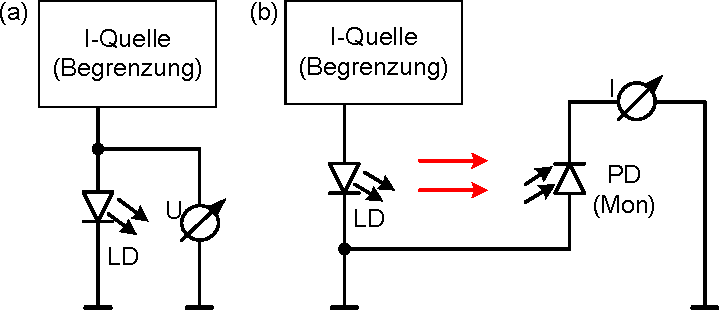
\includegraphics[width=.6\columnwidth]{Grafiken/measurement1.pdf}%
\caption{}%
\label{fig:measurement1}%
\end{figure}


\section{Recording of the U/I-Curve}

\begin{figure}%
\centering
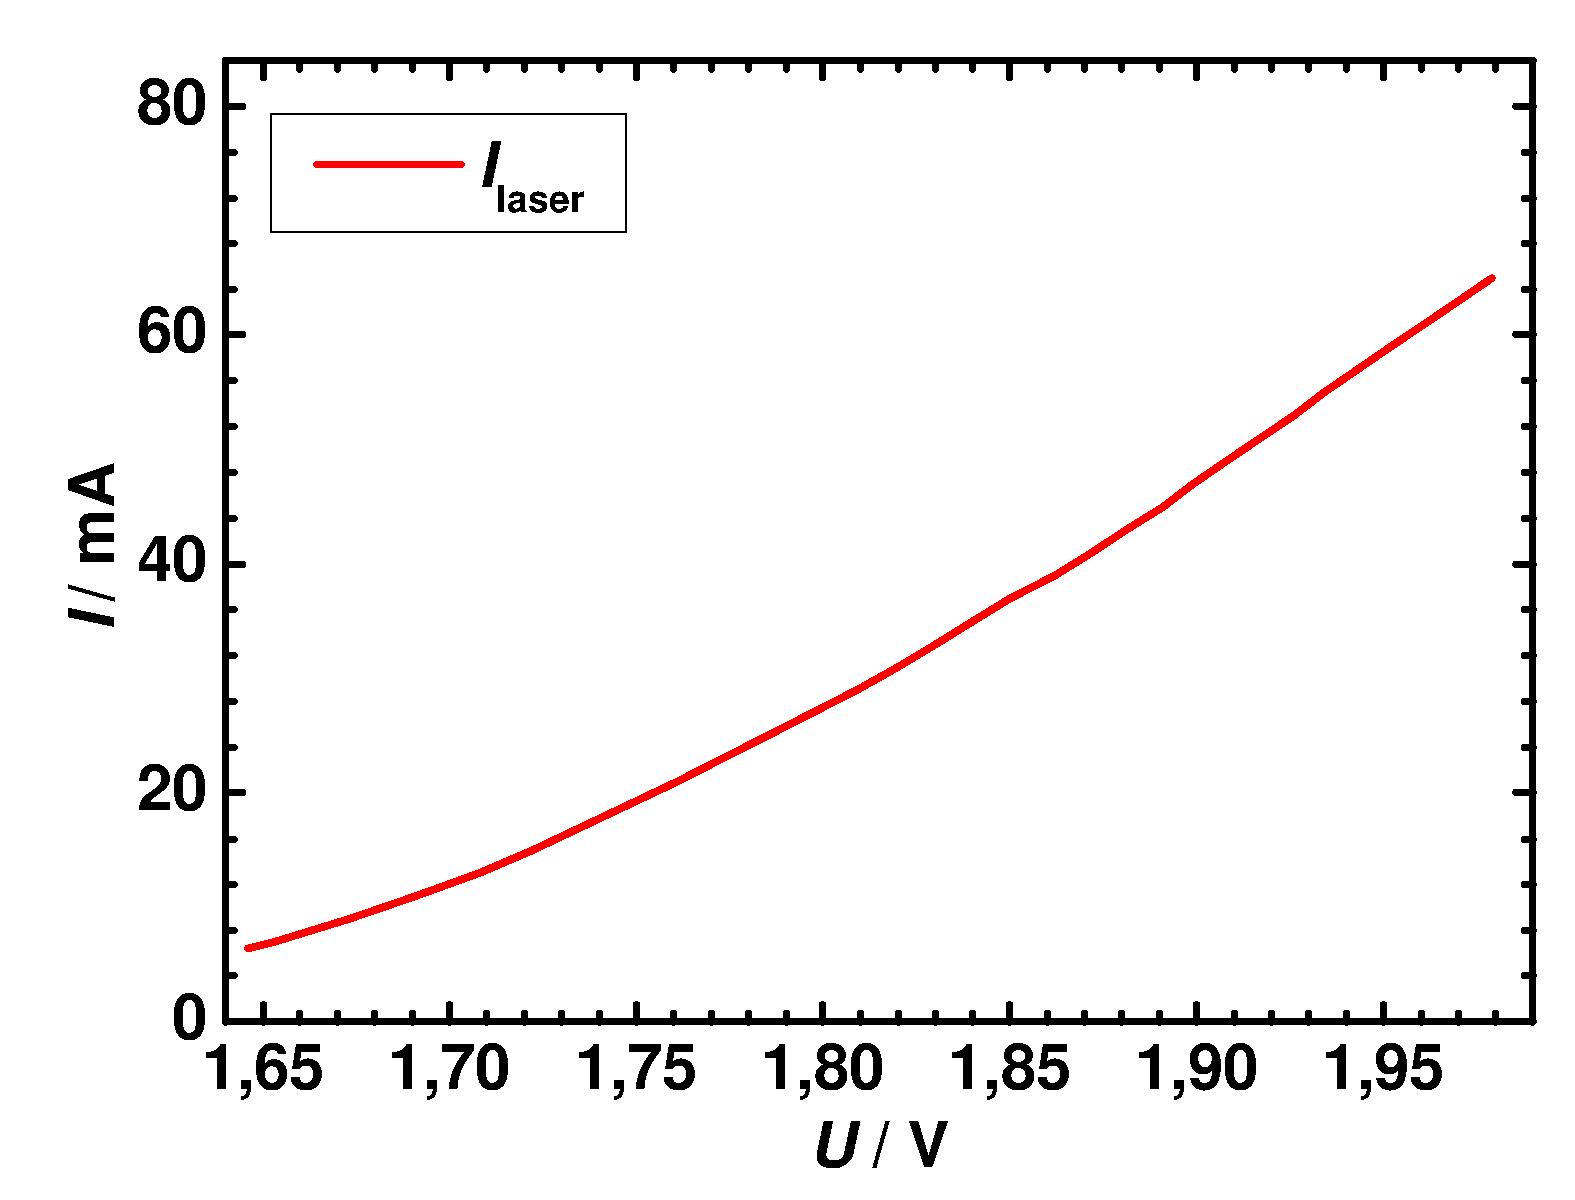
\includegraphics[width=.5\columnwidth]{Grafiken/1_IU.pdf}%
\caption{measured I/U curve at $T$~=~20~�C}%
\label{fig:1_IU}%
\end{figure}

 In the first experimental task the U/I-curve of the laser diode is recorded. This is done by biasing the diode with a current and measuring the voltage (cf. Figure \ref{fig:measurement1}a). The bias current is increased from a minimum of 6.4~mA to 65~mA in steps of 2~mA. The resulting $U/I$-curve is shown in Figure \ref{fig:1_IU}.

From
\begin{equation}
 \begin{split}
I = I\i{S0}\left[\e^{\beta\left(U-R\i{s}I\right)}-1\right] \hspace{2cm} I\leq I\i{S}\\
U = W\i{G}/e +R\i{S}I \hspace{2cm} I\geq I\i{S}\\
 \end{split}
\end{equation}
follows for the current above threshold:
\begin{equation}
 I = \frac{W\i{G}/e}{R\i{S}}-\frac{U}{R\i{S}}% = a + b\cdot U
 \label{eq:I/U}
\end{equation}
%The coefficients a and b can be determined by fitting a linear function to the U/I-curve above the threshold. The threshold current is calculated later in section \ref{ch:threshold}.  With these coefficients the band gap and the serial resistance of the laser diode can be calculated as:
\comwo{Mir ist nicht klar, wof�r du den linearen Fit brauchst. Ich habe das jetzt mal auskommentiert. Ich habe einfach in die �ber dem kommentar stehende Formel zwei messwerte weit oberhalb der Threshold-Spannung eingesetzt und damit dann zwei gleichungen aufgestellt}

Inserting two values of the linear range above threshold ($U(65~\mathrm{mA})=1.979~\mathrm{V}$ and $U(59~\mathrm{mA})=1.952~\mathrm{V}$) into \eqref{eq:I/U} leads to two equation which can be solved for $W\i{G}$ and $R\i{S}$:
\begin{equation}
\begin{split}
 W\i{G}=1.6865~\mathrm{eV}\\
 R\i{S} = 4.5~\Omega
\end{split}
\end{equation}
The bandgap of 1.6 corresponds to a wavelength of $\lambda =~$736~nm using 
Using 
\begin{equation}
W\i{G}=\frac{hc}{\lambda\i{G}}
\label{eq:}
\end{equation}
the to the bandgap corresponding wavelength can be calculated: 
\begin{equation}
\lambda\i{G}=736~\mathrm{nm}\quad.
\label{eq:lambda}
\end{equation}


\section{P/I-Curve}
The output power of the laser diode at different driving currents is measured with a reference detector at the rear mirror of the laser resonator. Because the reflectivity is the same at both mirrors of the laser diode, the measured power is identical with the power emmitted in the other direction. The setup for measuring is shown in figure \ref{fig:measurement1}b.
\begin{figure}%
\centering
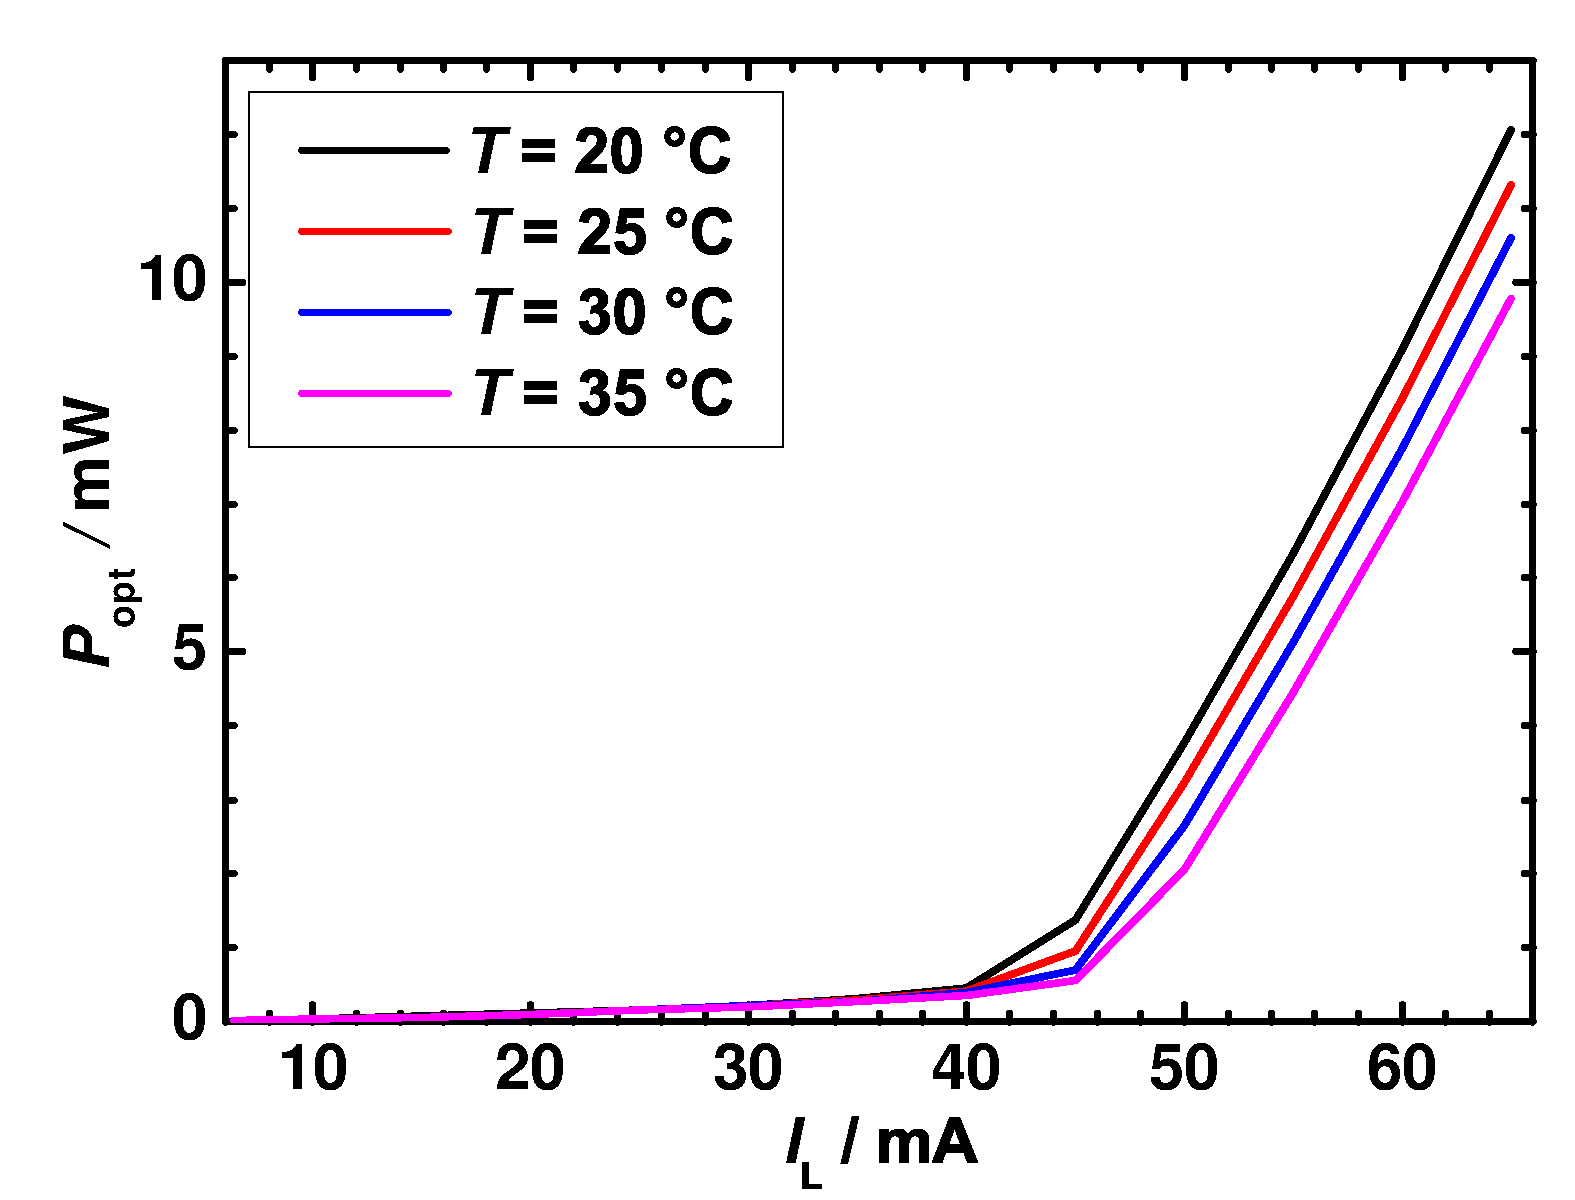
\includegraphics[width=.5\columnwidth]{Grafiken/2_PI.pdf}%
\caption{Optical power at the photodiode in dependence of the laser current and the temperature.}%
\label{fig:2_PI}%
\end{figure}

Figure \ref{fig:2_PI} shows the power-current characteristic of the laser diode for different temperatures. The power $P\i{opt}$ is the power that is received by the photo diode and therefore emitted at one side of the laser. One can see, that the characteristics shifts to higher currents for an increasing temperature.

The different threshold currents for the temperatures can be estimated by using a linear approximation of the $P/I$-curve for $I > I\i{th}$. The intersection of this linear approximation with the $I\i{L}$-axis is the estimated value of $I\i{th}$. Table \ref{tab:2_temp} shows the estimated values of $I\i{th}$ for the different temperatures.

\begin{table}%
\centering
\caption{Threshold currents for different temperatures.}
 
\begin{tabular}{cc}

\toprule
$T$~/~�C& $I\i{th}$~/~mA\\
\midrule

20&42.8\\
25&43.5\\
30&45.1\\
35&46.2\\
\bottomrule 
\end{tabular}
\label{tab:2_temp}
\end{table}

Using 
\begin{equation}
\begin{split}
I\i{th}(\Delta T)=I\i{th}(0)\mathrm{e}^{\frac{\Delta T}{T_0}}\\
\frac{\Delta T}{\mathrm{ln}(\frac{I\i{th}(\Delta T)}{I\i{th}(0)})}=T_0
\label{eq:2_T0}
\end{split}
\end{equation}
with the change of temperature $\Delta T$ and $I\i{th}$ is the threshold current before the temperature change the characteristic temperature $T_0$ can be found from measurements.

For the measured values $T_0$ is between
\begin{equation}
138~\mathrm{K} < T_0 < 310~\mathrm{K}\quad.
\label{eq:}
\end{equation}
\comwo{Hier bekomm ich f�r unterschiedliche eingesetze werte unterschiedliche $T_0$ raus.  Den H�chsten wert bekomm ich wenn ich 20�C und 25�C nutze., den niedrigsten wenn ich 25� und 30� benutz. :-/}

To calculate the external quantum efficiency 
\begin{equation}
\eta\i{ext}=\frac{P\i{a}/(hf)}{I/e}
\label{eq:}
\end{equation}
can be used.
$P\i{a}$ is the total output power of the laser diode. Since the mirrors at both sides of the laserdiode have the same reflectivity and therefore the same output powers. This leads to the total output power of  $P\i{a} = 2\cdot P\i{opt}$.

For $I = 60$~mA, $T = 20$~�C and $\lambda=736~\mathrm{nm}$ (cf. \eqref{eq:lambda}) an external quantum efficiency of $\eta\i{ext}=0.22$ can be calculated. 
\comwo{Hier h�ngt der wirkungsgrad massiv vom strom ab. Als wellenl�nge habe ich den zuvor bestimmten wert genommen}

The differential quantum efficiency 
\begin{equation}
\eta\i{d}=\frac{\mathrm{d}\left(\frac{P\i{a}}{hf}\right)}{\mathrm{d}\left(\frac{I}{e}\right)}
\label{eq:}
\end{equation}
is calculated to be
\begin{equation}
\eta\i{d} = 0.655~\mathrm{mW/mA}
\label{eq:}
\end{equation} at $T=20~$�C and currents above threshold.
\comwo{Einheit? Freude schreibt keine Einheit dahinter, das Datasheet gibt die Einheit an, die ich auch geschrieben hab}

To calculate the efficiency of the induced emission the values of the preparation for $\tau\i{P}$ (cf. \eqref{eq:tau_p}) and $\tau\i{R}$ (cf. \eqref{eq:tau_r}) are used.

\begin{equation}
\eta\i{ind}=\eta\i{d}\frac{\tau\i{R}}{\tau\i{P}}
\label{eq:}
\end{equation}
leads to $\eta\i{ind}$~=~1.28.
\comwo{Gr��er als 1. da kann was nicht stimmen! \\alternative vorgehensweise:}

\begin{equation}
\begin{split}
\eta\i{ind}=\eta\i{d}\frac{\eta\i{int}}{\eta\i{ext}}\\
=\eta\i{d}\frac{P}{P\i{a}}=\eta\i{d}\frac{UI-R\i{s}I^2}{2P\i{opt}}\\
=2.98
\end{split}
\label{eq:}
\end{equation}
for $I = 65$~mA and $U = 1.975$~V at $T = 20$~�C.

To calculate the number of photons above threshold neglecting spontaneous emission 
\begin{equation}
N\i{P}=\tau\i{P}\frac{I-I\i{th}}{e}
\label{eq:}
\end{equation}
can be used.
For $I = 65$~mA:
\begin{equation}
\begin{split}
N\i{P}(20~\mathrm{�C})\approx 245 \\
N\i{P}(30~\mathrm{�C})\approx 220
\end{split}
\label{eq:}
\end{equation}


 


\section{Modulation of the Laser Diode}

Now the photo diode is modulated with a frequency. This is done with a network analyzer (NWA). The modulation frequency is sweapt from 300~kHz to 3~GHz and the Output power is measured. By comparing the Power on the output to the input power, the frequency response of the transmission is determined. The setup of this experiment is shown in figure \ref{fig:measurement3}. Since the measurement PC was not working the frequency response had to be sketched by hand (cf. appendix \ref{}). 

The measurement of the frequency response was performed at different current levels the frequency $f\i{Kl}$ and the absolute of the frequency overshoot $\left|H\i{Kl}(f\i{Kl})/H\i{Kl}(0)\right|$ was recorded (cf. Tabular \ref{tab:} in the appendix). With  these values and the equations \eqref{eq:kleinsignal} and \eqref{eq:maximum} the parameters $\omega\i{r}^2$ and $\gamma\i{r}$ in dependency of the diode current $I_0$ can be calculated.  


% 
% Like described in the preparation material\todo{footnote}, the for the measured frequency response the hole transmission channel has to be taken into account. 

